\documentclass[12pt, a4paper]{article}

% ── Packages ──────────────────────────────────────────────────────
\usepackage{fontspec}
\setmainfont{Sylfaen}
\usepackage{amsmath, amssymb, amsthm}
\usepackage{mathtools}
\usepackage{enumitem}
\usepackage{tikz}
\usetikzlibrary{calc, positioning, arrows.meta, fit, patterns, decorations.pathreplacing}
\usepackage{geometry}
\geometry{margin=2.4cm}
\usepackage{xcolor}
\usepackage{tcolorbox}
\tcbuselibrary{theorems, skins, breakable}
\usepackage{booktabs}
\usepackage{hyperref}
\hypersetup{colorlinks=true, linkcolor=blue!60!black, urlcolor=blue!60!black}

\setlength{\parindent}{0pt}
\setlength{\parskip}{6pt}

% ── Colours ───────────────────────────────────────────────────────
\definecolor{setA}{RGB}{66, 133, 244}   % blue
\definecolor{setB}{RGB}{234, 67, 53}    % red
\definecolor{setC}{RGB}{251, 188, 4}    % yellow
\definecolor{theoryBg}{RGB}{232, 245, 253}
\definecolor{theoryFrame}{RGB}{66, 133, 244}
\definecolor{stmtBg}{RGB}{255, 243, 224}
\definecolor{stmtFrame}{RGB}{230, 126, 34}
\definecolor{ansBg}{RGB}{232, 250, 232}
\definecolor{ansFrame}{RGB}{39, 174, 96}

% ── Environments ──────────────────────────────────────────────────
\newtcolorbox{theorybox}[1][]{%
  colback=theoryBg, colframe=theoryFrame,
  fonttitle=\bfseries, title={\small Տեսության ամփոփում. #1},
  breakable, enhanced, arc=2mm,
  left=5pt, right=5pt, top=5pt, bottom=5pt
}

\newtcolorbox{problembox}{%
  colback=stmtBg, colframe=stmtFrame,
  fonttitle=\bfseries, title={\small Խնդրի դրվածք},
  breakable, enhanced, arc=2mm,
  left=5pt, right=5pt, top=5pt, bottom=5pt
}

\newtcolorbox{answerbox}{%
  colback=ansBg, colframe=ansFrame,
  arc=2mm, left=5pt, right=5pt, top=3pt, bottom=3pt
}

\newcommand{\Z}{\mathbb{Z}}
\newcommand{\R}{\mathbb{R}}
\newcommand{\N}{\mathbb{N}}
\newcommand{\powset}[1]{2^{#1}}
\newcommand{\comp}[1]{\overline{#1}}
\newcommand{\symdiff}{\mathbin{\triangle}}

% ── Title ─────────────────────────────────────────────────────────
\title{\textbf{Գործնական 6 — Զուգորդություններ և Նյուտոնի երկանդամ}\\[4pt]
       \large Ընտրված խնդիրների լուծումներ\\[2pt]
       \normalsize Խնդիրներ 8, 9, 11}
\author{Դիսկրետ մաթեմատիկա — ԵՊՀ}
\date{}

\begin{document}
\maketitle
\tableofcontents
\newpage

% ══════════════════════════════════════════════════════════════════
\section{Խնդիր 8 — Ցանցային ճանապարհներ՝ տրված կետի անցումով}
% ══════════════════════════════════════════════════════════════════

\begin{theorybox}[Ցանցային ճանապարհներ և Զուգորդություններ]
\textbf{Ցանցային ճանապարհը} $(0,0)$-ից մինչև $(m,n)$ բաղկացած է ճիշտ $m$ քայլ
դեպի աջ (R) և $n$ քայլ դեպի վեր (U), ցանկացած հերթականությամբ։
Քայլերի ընդհանուր քանակը $m + n$ է, և մենք պետք է ընտրենք, թե որ $m$ քայլերն են
R-քայլեր (մնացածը U-քայլեր են)․
\[
  (0,0)\text{-ից }(m,n)\text{ ճանապարհների քանակը}
  = \binom{m+n}{m} = \binom{m+n}{n}։
\]

\medskip
\textbf{Ճանապարհներ միջանկյալ կետով.}\;
Եթե ճանապարհը պետք է անցնի $P(p,q)$ կետով $O(0,0)$-ից $A(m,n)$ գնալիս
(որտեղ $0 \le p \le m$ և $0 \le q \le n$), մենք ճանապարհը բաժանում ենք
երկու անկախ հատվածների․
\[
  O \to P:\; \binom{p+q}{p} \text{ ճանապարհ},
  \qquad
  P \to A:\; \binom{(m-p)+(n-q)}{m-p} \text{ ճանապարհ}։
\]
Ըստ \textbf{արտադրյալի կանոնի}, ընդհանուր քանակը անկախ հատվածների արտադրյալն է։

\begin{center}
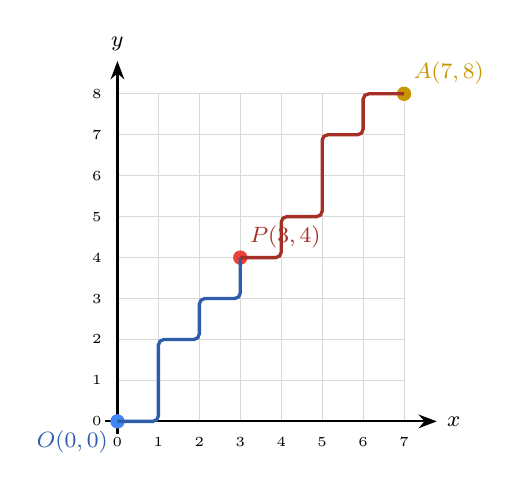
\begin{tikzpicture}[scale=0.52, >=Stealth, font=\small]
  % Grid
  \draw[gray!30] (0,0) grid (7,8);
  \draw[->, thick] (-0.3,0) -- (7.8,0) node[right, font=\footnotesize]{$x$};
  \draw[->, thick] (0,-0.3) -- (0,8.8) node[above, font=\footnotesize]{$y$};

  % Axis labels
  \foreach \x in {0,...,7}
    \node[below, font=\tiny] at (\x, -0.15) {$\x$};
  \foreach \y in {0,...,8}
    \node[left, font=\tiny] at (-0.15, \y) {$\y$};

  % Points
  \fill[setA] (0,0) circle (5pt);
  \node[below left, font=\footnotesize\bfseries, setA!70!black] at (0,0) {$O(0,0)$};

  \fill[setB] (3,4) circle (5pt);
  \node[above right, font=\footnotesize\bfseries, setB!70!black] at (3,4) {$P(3,4)$};

  \fill[setC!80!black] (7,8) circle (5pt);
  \node[above right, font=\footnotesize\bfseries, setC!80!black] at (7,8) {$A(7,8)$};

  % Sample path O -> P
  \draw[very thick, setA!70!black, rounded corners=2pt]
    (0,0) -- (1,0) -- (1,1) -- (1,2) -- (2,2) -- (2,3) -- (3,3) -- (3,4);

  % Sample path P -> A
  \draw[very thick, setB!70!black, rounded corners=2pt]
    (3,4) -- (4,4) -- (4,5) -- (5,5) -- (5,6) -- (5,7) -- (6,7) -- (6,8) -- (7,8);
\end{tikzpicture}
\end{center}
\end{theorybox}

\begin{problembox}
Գտեք $O(0,0)$ կետից $A(7,8)$ կետը տանող ցանցային ճանապարհների քանակը,
որոնք անցնում են $P(3,4)$ կետով։
\end{problembox}

\subsection*{Լուծում}

Ճանապարհը տրոհում ենք երկու անկախ հատվածի $P(3,4)$ կետում։

\textbf{Հատված 1: $O(0,0) \to P(3,4)$}\;
Պետք է 3 քայլ աջ և 4 քայլ վեր, ընդհանուր 7 քայլ։
Ընտրում ենք 3 աջ-քայլերը (կամ 4 վեր-քայլերը)․
\[
  \binom{3+4}{3} = \binom{7}{3}
  = \frac{7!}{3!\cdot 4!}
  = \frac{7 \cdot 6 \cdot 5}{3 \cdot 2 \cdot 1}
  = 35։
\]

\textbf{Հատված 2: $P(3,4) \to A(7,8)$}\;
$(3,4)$-ից $(7,8)$ հասնելու համար պետք է $7-3=4$ քայլ աջ և $8-4=4$ քայլ վեր,
ընդհանուր 8 քայլ։ Ընտրում ենք 4 աջ-քայլերը․
\[
  \binom{4+4}{4} = \binom{8}{4}
  = \frac{8!}{4!\cdot 4!}
  = \frac{8 \cdot 7 \cdot 6 \cdot 5}{4 \cdot 3 \cdot 2 \cdot 1}
  = 70։
\]

\textbf{Արտադրյալի կանոն.}\;
Երկու հատվածները անկախ են (առաջին հատվածի ցանկացած ճանապարհ կարող է
շարունակվել երկրորդ հատվածի ցանկացած ճանապարհով), ուստի․
\[
  \text{Ընդհանուր ճանապարհներ} = 35 \times 70 = 2450։
\]

\begin{answerbox}
\centering
$O(0,0)$-ից $A(7,8)$ տանող և $(3,4)$-ով անցնող ցանցային ճանապարհների
քանակն է $\binom{7}{3} \cdot \binom{8}{4} = 35 \cdot 70 = \boxed{2450}$։
\end{answerbox}

% ══════════════════════════════════════════════════════════════════
\newpage
\section{Խնդիր 9 — 6-ի տրոհումը երեք գումարելիների}
% ══════════════════════════════════════════════════════════════════

\begin{theorybox}[Աստղեր և գծիկներ / Թվի կոմպոզիցիաներ և տրոհումներ]
\textbf{Աստղեր և գծիկներ} (կրկնություններով զուգորդություններ).\;
\[
  x_1 + x_2 + \cdots + x_k = n, \qquad x_i \ge 0,
\]
հավասարման ոչ բացասական ամբողջական լուծումների քանակը
$\displaystyle\binom{n+k-1}{k-1}$ է։

\medskip
Եթե պահանջվում է $x_i \ge 1$ (դրական ամբողջ թվեր), տեղադրում ենք $y_i = x_i - 1 \ge 0$
և ստանում $y_1 + \cdots + y_k = n - k$, ինչը տալիս է
$\displaystyle\binom{n-1}{k-1}$ լուծում։

\medskip
\textbf{Թվի տրոհումներ (Integer partitions)} (չկարգավորված).\;
$n$ թվի տրոհումը $k$ մասերի դա $n$-ի ներկայացումն է
$n = \lambda_1 + \lambda_2 + \cdots + \lambda_k$ տեսքով, որտեղ
$\lambda_1 \ge \lambda_2 \ge \cdots \ge \lambda_k \ge 1$։
Կարգը էական չէ, այսինքն՝ $4+1+1$ և $1+4+1$ համարվում են \emph{նույն} տրոհումը։
\end{theorybox}

\begin{problembox}
Գտեք 6 թիվը երեք գումարելիների տրոհելու եղանակների քանակը։
\end{problembox}

\subsection*{Լուծում}

\textbf{Երկիմաստության նշում.}\; «Տրոհել երեք գումարելիների» կարող է նշանակել կարգավորված (կոմպոզիցիաներ) կամ չկարգավորված (բուն տրոհումներ)։ Մենք կլուծենք երկու տարբերակն էլ։

\subsubsection*{Տարբերակ 1: Կարգավորված գումարելիներ (կոմպոզիցիաներ)}

Փնտրում ենք հետևյալ հավասարման լուծումների քանակը․
\[
  x_1 + x_2 + x_3 = 6, \qquad x_i \ge 1.
\]
Ըստ աստղերի և գծիկների բանաձևի ($y_i = x_i - 1$ տեղադրմամբ)․
\[
  \binom{6-1}{3-1} = \binom{5}{2} = \frac{5!}{2!\cdot 3!} = 10.
\]

\begin{center}
\renewcommand{\arraystretch}{1.15}
\begin{tabular}{cccc}
\toprule
\textbf{\#} & $x_1$ & $x_2$ & $x_3$ \\
\midrule
1  & 4 & 1 & 1 \\
2  & 1 & 4 & 1 \\
3  & 1 & 1 & 4 \\
4  & 3 & 2 & 1 \\
5  & 3 & 1 & 2 \\
6  & 2 & 3 & 1 \\
7  & 1 & 3 & 2 \\
8  & 2 & 1 & 3 \\
9  & 1 & 2 & 3 \\
10 & 2 & 2 & 2 \\
\bottomrule
\end{tabular}
\end{center}

\subsubsection*{Տարբերակ 2: Չկարգավորված գումարելիներ (տրոհումներ)}

Փնտրում ենք $6 = \lambda_1 + \lambda_2 + \lambda_3$ ներկայացումների քանակը,
որտեղ $\lambda_1 \ge \lambda_2 \ge \lambda_3 \ge 1$։

Թվարկենք բոլոր հնարավորությունները․
\begin{center}
\renewcommand{\arraystretch}{1.15}
\begin{tabular}{cl}
\toprule
\textbf{\#} & \textbf{Տրոհում} \\
\midrule
1 & $4 + 1 + 1$ \\
2 & $3 + 2 + 1$ \\
3 & $2 + 2 + 2$ \\
\bottomrule
\end{tabular}
\end{center}

Կա ճիշտ \textbf{3} այդպիսի տրոհում։

\begin{answerbox}
\centering
\textbf{Կարգավորված} (կոմպոզիցիաներ դրական մասերով)՝
$\displaystyle\binom{5}{2} = 10$ եղանակ։\\[4pt]
\textbf{Չկարգավորված} (տրոհումներ 3 մասի)՝
$3$ եղանակ՝ \;$4{+}1{+}1$,\; $3{+}2{+}1$,\; $2{+}2{+}2$։
\end{answerbox}

% ══════════════════════════════════════════════════════════════════
\newpage
\section{Խնդիր 11 — «մաթեմատիկա» բառի վերադասավորումները}
% ══════════════════════════════════════════════════════════════════

\begin{theorybox}[Պոլինոմիալ գործակից / Տեղափոխություններ կրկնությամբ]
Եթե ունենք $n$ օբյեկտ, որտեղ կան $k$ տարբեր տեսակներ $n_1, n_2, \ldots, n_k$
քանակներով (այնպես որ $n_1 + n_2 + \cdots + n_k = n$), ապա տարբեր
դասավորությունների քանակը հավասար է \textbf{պոլինոմիալ գործակցին}․
\[
  \binom{n}{n_1,\, n_2,\, \ldots,\, n_k}
  = \frac{n!}{n_1!\cdot n_2!\cdots n_k!}։
\]

\medskip
\textbf{Իմաստը.}\;
Սկսում ենք $n!$ դասավորություններից (կարծես բոլոր տառերը տարբեր են),
ապա բաժանում ենք $n_i!$-ի յուրաքանչյուր նույնական տառի խմբի ներքին տեղափոխությունների համար։
\end{theorybox}

\begin{problembox}
Քանի՞ տարբեր բառ կարելի է կազմել՝ վերադասավորելով \textbf{«matematika»} բառի բոլոր տառերը։
\end{problembox}

\subsection*{Լուծում}

\textbf{Քայլ 1. Հաշվել տառերը և դրանց հաճախականությունները.}

«matematika» բառում կան հետևյալ տառերը․
\[
  \text{m -- a -- t -- e -- m -- a -- t -- i -- k -- a}
\]
Ընդհանուր $n = 10$ տառ։ Հաշվենք յուրաքանչյուրը․

\begin{center}
\renewcommand{\arraystretch}{1.2}
\begin{tabular}{lcccccc}
\toprule
\textbf{Տառ} & a & m & t & e & i & k \\
\midrule
\textbf{Քանակ} $n_i$ & 3 & 2 & 2 & 1 & 1 & 1 \\
\bottomrule
\end{tabular}
\end{center}

\textbf{Ստուգում.}\; $3 + 2 + 2 + 1 + 1 + 1 = 10$ \;\checkmark

\medskip
\textbf{Քայլ 2. Կիրառել պոլինոմիալ գործակիցը.}

\[
  \frac{10!}{3!\cdot 2!\cdot 2!\cdot 1!\cdot 1!\cdot 1!}
  = \frac{10!}{3!\cdot 2!\cdot 2!}
\]

Հաշվարկ․
\begin{align*}
  10! &= 3\,628\,800, \\
  3! \cdot 2! \cdot 2! &= 6 \cdot 2 \cdot 2 = 24, \\[4pt]
  \frac{3\,628\,800}{24} &= 151\,200.
\end{align*}

\begin{answerbox}
\centering
«matematika» բառի տարբեր վերադասավորումների քանակն է
$\displaystyle\frac{10!}{3!\cdot 2!\cdot 2!} = \boxed{151\,200}$։
\end{answerbox}

\end{document}